%%%%%%%%%%%%%%%%%%%%%%%%%%%%%%%%%%%%%%%%%%%%%%%%%%%%%%%%%%%%%%%%%%%%%%
% Reverted to tufte-handout with [nols] to fix soul package errors
%%%%%%%%%%%%%%%%%%%%%%%%%%%%%%%%%%%%%%%%%%%%%%%%%%%%%%%%%%%%%%%%%%%%%%
%! TEX program = lualatex
\documentclass[no-fonts,nols]{tufte-handout} 

\usepackage{stmaryrd}
\usepackage{amsmath}
\usepackage{euler-math}

% ------------------------- 
\usepackage{fontspec}
\setmainfont{CMU Concrete}
\setsansfont{CMU Sans Serif}
\setmonofont{CMU Typewriter Text}
% -------------------------
   
\usepackage{tikz}
\usetikzlibrary{arrows.meta, positioning}

\usepackage{graphicx}
\setkeys{Gin}{width=\linewidth,totalheight=\textheight,keepaspectratio}
\graphicspath{{graphics/}}

\title{Full-Index Notation Considered Better}
\author{Brian Beckman}

\usepackage{booktabs}
\usepackage{siunitx}
\usepackage{fancyvrb}
\fvset{fontsize=\normalsize}
\usepackage{multicol}
\usepackage{lipsum}

\begin{document}

\maketitle

\begin{abstract} \noindent Index-free notation is very popular.
	However, it fails to distinguish syntactically between types.
	This failure challenges static type checking of expressions
	like $\symbf{v}+\symbf{k}$. Is this a nonsensical addition of
	a vector to a 1\nobreakdash-form, or, even worse, a vector
	added to a 2\nobreakdash-form? In this note, we argue that,
	at least for symbolic computing and automated
	theorem-proving, the older, full-index notation is superior,
	being unambiguous yet not giving up much brevity. 
\end{abstract}

\noindent In index-free notation, one typically writes contravariant
vectors in bold Latin, as in $\symbf{v}$, and covariant covectors in
bold Greek, as in $\symbf{\omega}$ (see, for instance, Part II of
MTW\cite{MTW2017}). The argument for index-free notation is that
geometric objects exist independently of particular choice of
coordinates. However, I argue that such objects do not exist
independently of \textit{any} coordinates. One must ultimately choose
\textit{some} coordinates, and, no matter what coordinates one
chooses, the dimensionality, or number of index values for each
index, is the same. Once a coordinate system is chosen, one might as
well denote a vector, for instance, by its coordinate tuple $v^\mu$
as by its index-free symbol $\symbf{v}$. The tuple notation is not
much longer, yet is totally unambiguous. There are further benefits
to full-index notation (despite its being considered
old-fashioned).\cite{lovelock1989tensors} To summarize:

\begin{enumerate} 

	\item It honors the fact that \textit{some} coordinates must
		be chosen.

	\item It honors the fact that all coordinate systems have the
		same dimensionality; 4 in the case of relativistic
		spacetime.

	\item It distinguishes contravariant (up) indices from
		covariant (down) indices, empowering type checking
		and tracking of \textit{valence} (up-down pattern) of
		expressions.

	\item Is is friendly to Einsteim-summation, so a
		compiler\cite{RelativityToolkit} can check
		expressions like $v_{\mu}=g_{\mu\nu}v^{\nu}$.

\end{enumerate}

\noindent In the rest of this note, I present motivation about why
tracking valence is crtical, plus some handy mnemonics for some
cases.

\section{Valence: Contravariance and Covariance}

Imagine two coordinate systems or \textit{gauges} over spacetime:
$X$, measuring distances in inches, and ${X'}$, measuring distances
in feet. $X$ is a set of real 4\nobreakdash-tuples,
$x^\mu=(x^0,x^1,x^2,x^3)$, and $X'$ likewise,
${x'}^\mu=({x'}^0,{x'}^1,{x'}^2,{x'}^3)$,\sidenote{MTW put the
prime on the index, as in ${x}^{\mu'}$. Other authors, like us, put
the prime on the coordinate symbol, as in ${x'}^{\mu}$} with $\mu$ running from $0$
through $3$. Each is a copy of $\mathbb{R}^4$.

In physics, tuples like $x^\mu$ or ${x'}^\mu$ can locate any
point in spacetime, or can denote a measurement of 
the time and 3D spatial location of an event,
with time measured in distance units.\sidenote{
	Measure time in distance units by multiplying
	time by the universal constant, $c$, the speed of light, 
	which has the same values, one for each gauge, in all 
	inertial frames: 

    $c \approx 1.18 \times 10^{10}$~in/s and 

    $c' \approx 9.84 \times 10^{8}$~ft/s.}

Let $x^\mu$ denote a measurement of the spacetime location of some
event in $X$, in inches, and let ${x'}^{\mu}$ denote a measurement of
the spacetime location of the same event in $X'$, in feet (mnemonic:
remember that \textit{the prime} is in \textit{feet}). Dropping the
index,\sidenote{ironically} one might say $x=12 \times x'$ for any 
such matched pair of measurements.

Now imagine $\mu$ functions $x^\mu({x'}^{\nu})$ that, given a
measurement tuple, ${x'}^{\nu}$, in feet, produce components,
$x^\mu$, of a measurement of the location of the same event in
inches.\sidenote{We use the same symbol, $x^\mu$, for the
	coordinates of the event and for the functions that convert
measurements. This kind of
ambiguity is common in mathematics.}

For the following arguments, we can drop the
indices.\sidenote{ironically, again} Treating $x$ as a
coordinate-transformation function $x(x')$, we can compute its
partial derivative,\sidenote{In full flower, we would have the
16-element Jacobian matrix,
$\left.\partial{x^{\mu}}\middle/\partial{{x'}^{\nu}}\right.$} which,
of course, is also a function of the same independent variable, $x'$.
This partial derivative happens to be the constant, $12$, in our
example:

\newcommand{\dxdxprime}{\frac{\partial{x}}{\partial{x'}}}
\newcommand{\dxprimedx}{\frac{\partial{x'}}{\partial{x}}}

\begin{equation}
    \dxdxprime = 12 \qquad\text{(inches per foot)}
\label{eq:coordinateTransform}
\end{equation}

We always insist that our coordinate-transformation functions be
invertible and differentiable, so the inverse function $x'(x)$ exists
and has the partial derivative:

\begin{equation}
    \dxprimedx = \frac{1}{12} \qquad\text{(feet per inch)}
\end{equation}

Now, imagine another quantity, $v^\mu$, which measures velocity in
the $x$, or `inches,' gauge. We wish to know its value, ${v'}^{\mu}$,
in the `feet' gauge. We know the answer, hardly without thinking!

\begin{equation}
\begin{split}
	{v'}^{\mu}\:\text{(feet per second)} &= 
    \left. v^\mu\:\text{(inches per second)} 
    \middle/ 
    \dxdxprime \right. \\
	{v'}^{\mu} &= v^\mu {} \dxprimedx
\end{split}
\end{equation}

This is the definitional example of a \textbf{\textit{contravariant
quantity}}. A way to remember it is

\begin{equation}
    \left(\text{
        \begin{tabular}{c}
             quantity \\ measured in \\ primed \\ gauge 
        \end{tabular}
    }\right) = 
    \left(\text{
        \begin{tabular}{c}
            quantity \\ measured in \\ unprimed \\ gauge
        \end{tabular}
    }\right) 
    \frac{\partial{
            \left(\text{
                \begin{tabular}{c}
                     primed \\ gauge
                \end{tabular}
            }\right)
         }}
         {\partial{
            \left(\text{
                \begin{tabular}{c}
                     unprimed \\ gauge
                \end{tabular}
            }\right)
         }}
\end{equation}

i.e., the unprimed quantity on the right-hand side is multiplied by a
derivative with the unprimed gauge in the \textit{denominator}.

Now consider a quantity, $u_\mu$, measuring temperature gradient in
degrees per inch, and its partner in the other gauge, ${u'}_{\mu}$,
measuring the same temperature gradient, but in degrees per foot.
Again, we know the transformation almost without thinking:

\begin{equation}
\begin{split}
	{u'}_{\mu}\:\text{(degrees per foot)} &= 
    u_\mu\:\text{(degrees per inch)} 
    \times
    \dxdxprime \\
	{u'}_{\mu} &= u_\mu {} \dxdxprime
\end{split}
\end{equation}

This is the definitional example of a \textbf{\textit{coavariant
quantity}}. The way to remember it is

\begin{equation}
    \left(\text{
        \begin{tabular}{c}
             quantity \\ measured in \\ primed \\ gauge 
        \end{tabular}
    }\right) = 
    \left(\text{
        \begin{tabular}{c}
            quantity \\ measured in \\ unprimed \\ gauge
        \end{tabular}
    }\right) 
    \frac{\partial{
            \left(\text{
                \begin{tabular}{c}
                     unprimed \\ gauge
                \end{tabular}
            }\right)
         }}
         {\partial{
            \left(\text{
                \begin{tabular}{c}
                     primed \\ gauge
                \end{tabular}
            }\right)
         }}
\end{equation}

i.e., the unprimed quantity on the right-hand side is multiplied by a 
derivative with the unprimed gauge in the \textit{numerator}. 

A contravariant quantity like velocity is not compatible with a covariant
quantity like a gradient. Even though they both have four components, it 
makes no sense to add them. There are ways to transform one into the other, 
and ways to combine them via \textit{contraction}, but those take us afar
from the point of this short letter. The takeaway, here, is that we must 
distinguish them. If we're doing automatic computation, we should help the
computer distinguish them. The best way to do that is symbolically, hence
we conclude that explicit index notation is the way forward.

Finally, putting the indices back in, and assuming Einsteim-summation
(automatically sum over repeated indices in up-down
pairs)\sidenote{The Relativity Toolkit's (op. cit.) compiler
	automatically performs such sums and automatically renames
	indices to prevent index collision and capture.}, we offer
	the following, final cheat-sheet:

\begin{figure}
  \centering
  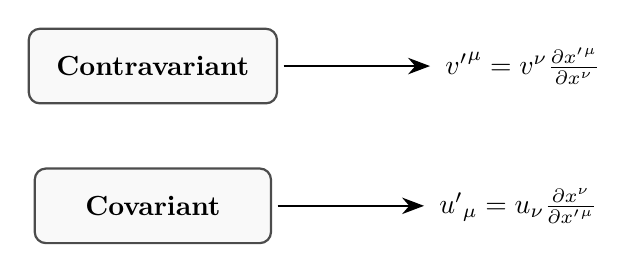
\begin{tikzpicture}[
    node distance=0.8cm and 2cm,
    box/.style={rectangle, draw=black!70, fill=gray!5, thick, 
    rounded corners, inner sep=10pt, minimum width=3cm},
    arrow/.style={-{Stealth[scale=1.2]}, thick, shorten >=2pt, 
    shorten <=2pt} ]

    % Nodes for Contravariant
    \node[box] (con_label) {\textbf{Contravariant}};
    \node[right=of con_label] (con_eq) 
	    {${v'}^{\mu} = v^{\nu} 
	    \frac{\partial {x'}^{\mu}}{\partial x^{\nu}}$};

    % Nodes for Covariant
    \node[box, below=of con_label] (cov_label) {\textbf{Covariant}};
    \node[right=of cov_label] (cov_eq) 
	    {${u'}_{\mu} = u_{\nu} 
	    \frac{\partial x^{\nu}}{\partial {x'}^{\mu}}$};

    % Arrows indicating the transformation rule
    \draw[arrow] (cov_label) -- (cov_eq);
    \draw[arrow] (con_label) -- (con_eq);

  \end{tikzpicture}
  \caption{Tensor transformation rules for 
           contravariant and covariant indices.}
  \label{fig:tensor_transform}
\end{figure}

\bibliography{sample-handout}
\bibliographystyle{plainnat}

\end{document}
